\documentclass{article}
\usepackage{graphicx}

\author{Christian M\"osl, 01523736}
\title{Aufgabe 3}
\date{}

\begin{document}
\maketitle

\paragraph{} 
Es sind 3 unterschiedliche Grafiken mit Gnuplot zu erstellen, welche auf der Studierendenstatistik der Uni Salzburg beruhen.
\vspace{1cm}

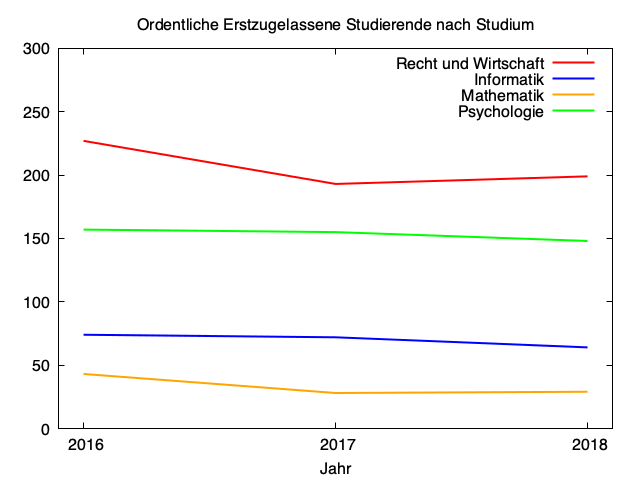
\includegraphics[width=12cm]{first-semester.png} \\
\vspace{1cm}
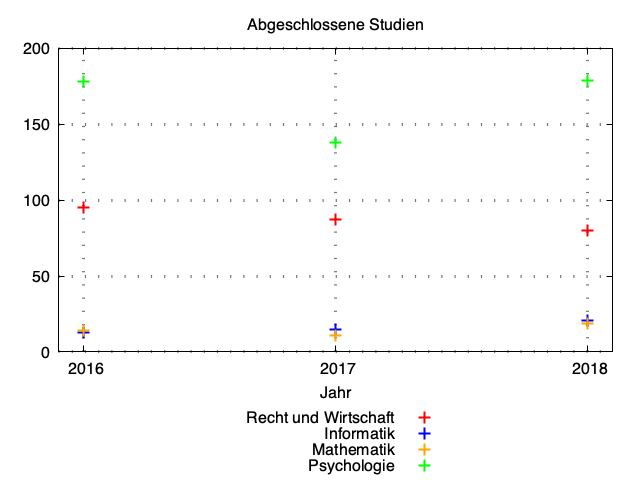
\includegraphics[width=12cm]{graduations.png} \\
\vspace{1cm}
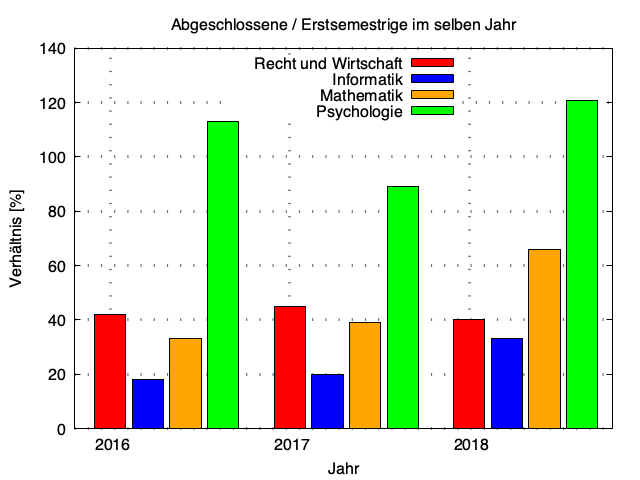
\includegraphics[width=12cm]{factor.png} \\

\end{document}
